\documentclass[conference]{IEEEtran}

%Packages
\usepackage[pdftex]{graphicx}
\usepackage{tabularx,ragged2e}
\usepackage{caption}
\usepackage{subcaption}
\title{Biomedical Image Segmentation Using CNN: A Survey}

%Document started from here
\begin{document}
	\author{\IEEEauthorblockN{Farhana Sultana}
		\IEEEauthorblockA{Department of Computer Science\\
			University of Gour Banga\\
			West Bengal, India\\
			Email: sfarhana@ieee.org}
		\and
		\IEEEauthorblockN{Abu Sufian}
		\IEEEauthorblockA{Department of Computer Science\\
			University of Gour Banga\\
			West Bengal, India\\
			Email: sufian@ieee.org}
		\and
		\IEEEauthorblockN{Paramartha Dutta}
		\IEEEauthorblockA{Department of CSS\\
			Visva-Bharati University\\
			West Bengal, India\\
			%Santiniketan,West Bengal ,India\\
			Email: paramartha.dutta@gmail.com}}
	
	
	\IEEEoverridecommandlockouts
	%Define custom IEEEpubid that will place it self in a column and not a page, suitable from conference class
	\IEEEpubid{\makebox[\columnwidth]{
			978-1-5386-7638-7/18/\$31.00~\copyright~2018 IEEE \hfill}
		\hspace{\columnsep}\makebox[\columnwidth]{ }}
	
	\maketitle

\begin{abstract}
	Convolutional Neural Network (CNN) is the state-of-the-art for image classification task. Here we have briefly discussed different components of CNN. In this paper, We have explained different CNN architectures for image classification. Through this paper, we have shown advancements in CNN from LeNet-5 to latest SENet model. We have discussed the model description and training details of each model. We have also drawn a comparison among those models. 
	
\end{abstract}

 \begin{IEEEkeywords}
	AlexNet, Capsnet, Convolutional Neural Network, Deep learning, DenseNet, Image classification, ResNet, SENet. 
\end{IEEEkeywords}

\section{Introduction}
Computer vision consists of different problems such as image classification, localization, segmentation and object detection. Among those, image classification can be considered as the fundamental problem and forms the basis for other computer vision problems. Until '90s only traditional machine learning approaches were used to classify image. But the accuracy and scope of the classification task were bounded by several challenges such as hand-crafted feature extraction process etc.
\section{Convolutional Neural Network}
A typical CNN is composed of single or multiple blocks of convolution and sub-sampling layers, after that one or more fully connected layers and an output layer as shown in figure \ref{fcnn}.

\begin{figure}[htb]
	\centering
	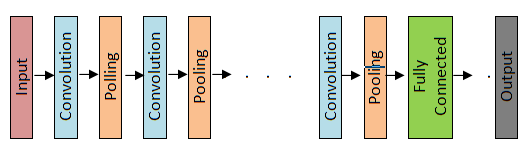
\includegraphics[scale=0.4 ]{image/CNN}
	\caption{Building block of a typical CNN}
	\label{fcnn}
\end{figure}

 \subsection{Convolutional Layer}
The convolutional layer (conv layer) is the central part of a CNN. Images are generally stationary in nature. That means the formation of one part of the image is same as any other part. So, a feature learnt in one region can match similar pattern in another region. In a large image, we take a small section and pass it through all the points in the large image (Input). While passing at any point we convolve them into a single position (Output). Each small section of the image that passes over the large image is called filter (Kernel). The filters are later configured based on the back propagation technique. Figure \ref{fconv_layer} shows typical convolutional operation.

\begin{figure}[htb]
	\centering
	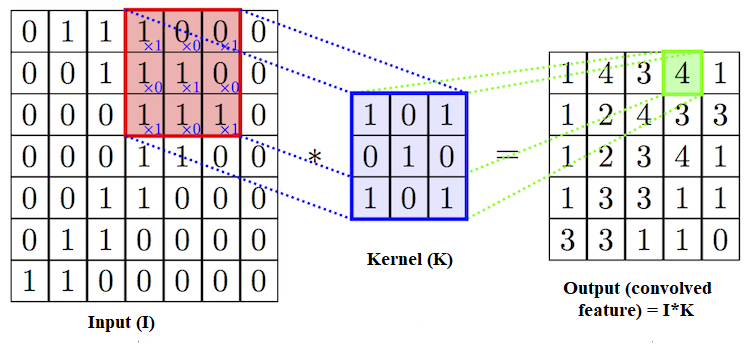
\includegraphics[scale=0.3]{image/Conv_layer}
	\caption{Convolutional Layer}
	\label{fconv_layer}
\end{figure}
%\subsection{Activation Layer}   
\subsection{Sub-sampling or Pooling Layer}
Pooling simply means down sampling of an image. It takes small region of the convolutional output as input and sub-samples it to produce a single output. Different pooling techniques are there such as max pooling, mean pooling, average pooling etc. Max pooling takes largest of the pixel values of a region as shown in figure \ref{fmax_pool}. Pooling reduces the number of parameter to be computed but makes the network invariant to translations in shape, size and scale.     
\begin{figure}[htb]
	\centering
	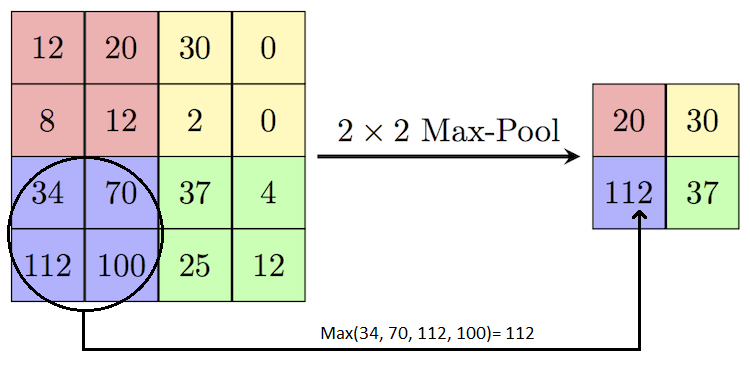
\includegraphics[scale=0.2 ]{image/max_pool}
	\caption{Max Pooling operation}
	\label{fmax_pool}
\end{figure}

\subsection{Fully-connected Layer (FC Layer)}
Last section of CNN are basically fully connected layers as depicted in figure \ref{ffclayer}. This layer takes input from all neurons in the previous layer and performs operation with individual neuron in the current layer to generate output. 

\begin{figure}[htb]
	\centering
	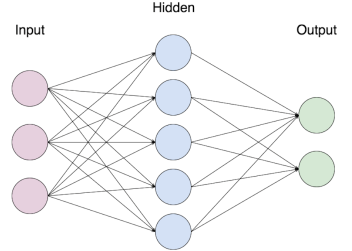
\includegraphics[scale=0.3 ]{image/fclayer}
	\caption{Fully-connected layer}
	\label{ffclayer}
\end{figure}


\begin{table}
\centering
\caption{Table to test captions and labels}
\label{table:1}
	\begin{tabular}{ |c|c|c|c| } 
		\hline
		 Heading1 &  Heading2 &  Heading3 & Heading4\\ \hline
		cell4 & cell5 & cell6&89.5\% \\ 
		cell7 & cell8 & cell9&93.9\% \\ 
		\hline
	\end{tabular}

\end{table}

\section{Conclusion}
In this study, we have discussed the advancements of CNN in image classification tasks. We have shown here that although AlexNet\cite{Alex2012}, ZFNet\cite{Zeiler2014} and VGGNet followed the architecture of conventional CNN model such as LeNet-5 their networks are larger and deeper. We have experienced that combining inception module and residual blocks with conventional CNN model, GoogLeNet and ResNet gained better accuracy than stacking the same building blocks again and again. DenseNet focused on feature reusing to strengthen the feature propagation. Though CapsNet reached state-of-the-art achievement on MNIST but it is yet to perform as well as previous CNNs performance on high resolution image dataset such as ImageNet. %But the key ideas of CapsNet are extremely promising towards the field of computer vision. 
The result of SENet on ImageNet dataset gives us the hope that it may turn out useful for other task which requires strong discriminative features.


\bibliographystyle{IEEEtran}

\bibliography{mybib}

\end{document}
